\section{Reasoning Output-based Efficient Reasoning}
From the perspective of reasoning steps in the output, these works focus on modifying the output paradigm to enhance the ability of LLMs to reason concisely and efficiently.

\subsection{Compressing Reasoning Steps into Fewer Latent Representation}
\label{sec:latent}


Although standard CoT methods improve LLM performance by explicitly writing reasoning steps, recent work~\cite{deng2024explicit} has shown that simply adding intermediate ``thinking'' tokens, or even meaningless filler (e.g., ``......'')~\cite{pfau2024let}, can also increase performance. \cite{geiping2025scaling} scales up deeper reasoning through recurrent expansions in the hidden space rather than verbose text. These findings highlight that the benefit often lies in more hidden computation rather than purely textual decompositions. Building on the insight that latent reasoning can allow LLMs to reason more efficiently and flexibly, \textit{with fewer (or no) explicit textual intermediate steps, several new methods focus on compressing or replacing explicit CoT with more compact latent representations.}

\insightbox{The key question is: How to compress reasoning steps into latent space?}

\begin{figure}[h]
    \centering
    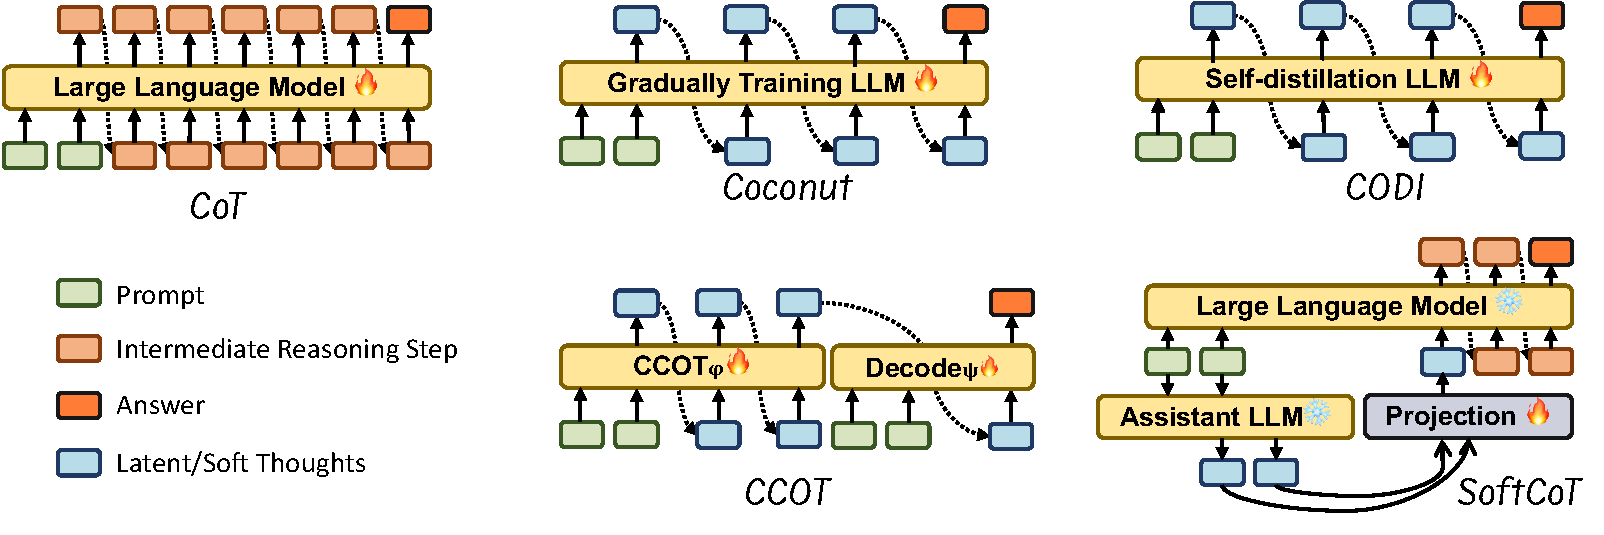
\includegraphics[width=\linewidth]{figs/latent.pdf}
    \caption{
    Comparison of methods of compressing reasoning steps into fewer latent representations.}
    \label{fig:latent}
\end{figure}

In general, these methods can be categorized into two types: training LLMs to inference using latent representations or using an auxiliary model. A visualized comparison of some of these approaches is presented in Figure~\ref{fig:latent}.

\paragraph{Training LLMs to Leverage Latent Representations.}
%
Among the first explorations, Coconut (Chain of Continuous Thought)~\cite{hao2024training} treats the final-layer hidden states of an LLM as ``continuous thought'' to replace traditional discrete tokens. It then reuses these hidden states as the next input embeddings. Trained step by step, Coconut gradually adds these latent CoT tokens. The results suggest that compressing tokens into latent representations improves both accuracy and efficiency by reducing the number of intermediate ``thinking'' tokens.
%
CODI~\cite{shen2025codi} leverages a different training process compared to Coconut, which learns the continuous latent CoT via \textit{self-distillation}. In CODI, the model serves both teacher and student, jointly learning explicit and implicit CoT while aligning hidden activations on the token, generating the final answer. This self-distillation process enables LLMs to perform reasoning internally without generating explicit CoT tokens.
%
Similarly, CCOT~\cite{cheng2024compressed} condenses long CoT reasoning into short \textit{contentful and continuous contemplation tokens}. First, it precomputes the full CoT for a query and selects the most important hidden states as a gold standard for compression. The CCOT module (a LoRA) is trained to predict these key tokens. Then, the DECODE module (another LoRA) is trained on the query plus compressed tokens. During inference, CCOT generates compressed tokens, which DECODE uses to produce concise reasoning steps. Another type of work, summarization-based dynamic reasoning, as mentioned in Section~\ref{sec:dynamic} explores compressing and summarizing reasoning steps in discrete space during inference, which is similar to the introduction of ``contemplation token''.

Another work, Heima~\cite{shen2025efficient}, inspired by Coconut~\cite{hao2024training}, brings latent reasoning into Multimodal Large Langue Models (MLLMs). Instead of always using full, lengthy reasoning explanations, Heima replaces each stage of detailed reasoning with a single ``thinking token''. With this change, the training data is updated. Instead of long textual explanations, each reasoning stage is just one of these thinking tokens. Then, they continue fine-tuning the model to achieve efficient reasoning.
%
Token Assorted~\cite{su2025token} adopts a hybrid approach. During training, part of the CoT is replaced by discrete latent tokens learned via a VQ-VAE~\cite{van2017neural}, and then the LLM is trained with a partial and high-level abstract of the reasoning steps. The authors show that mixing text tokens with latent tokens can facilitate training and inference by representing some reasoning steps in a compact latent form. 
%
Other than explicitly compressing the discrete tokens into latent space, \cite{saunshi2025reasoning} demonstrates that looping a $k$-layer transformer $L$ times can emulate the performance of a $kL$-layer model. This looping mechanism effectively increases the depth of the model depth without adding parameters, enabling iterative reasoning processes within the latent space. The study reveals that \textit{looped models implicitly generate latent thoughts}, allowing them to simulate multiple steps of CoT reasoning through successive loops.

\paragraph{Training Auxiliary Modules while Keeping LLMs Frozen.} 
%
While most methods for continuous-space reasoning fine-tune the pre-trained LLM, SoftCoT~\cite{xu2025softcot} keeps the underlying LLM frozen. A lightweight auxiliary model generates instance-specific soft thought tokens projected into the embedding space of the frozen LLM. Experiments show that SoftCoT consistently boosts performance, demonstrating the viability of augmenting LLMs with external latent reasoning tokens.

These methods hint at a broader move toward latent reasoning, where critical thinking occurs in compressed, non-textual forms. Such approaches can unlock improved speed, adaptive inference, parallel backtracking, and new ways to interpret or partially reveal the model reasoning. As LLMs grow larger and tasks become more complex, balancing thorough reasoning with computational efficiency is greatly beneficial from these flexible and compact latent CoT paradigms.